\usepackage{listings}  % 排代码用的宏包
\lstset{
    language = HTTP,
    backgroundcolor = \color{yellow!10},    % 背景色:淡黄
    basicstyle = \small\ttfamily,           % 基本样式 + 小号字体
    rulesepcolor= \color{gray},             % 代码块边框颜色
    breaklines = true,                  % 代码过长则换行
    numbers = left,                     % 行号在左侧显示
    numberstyle = \small,               % 行号字体
    keywordstyle = \color{blue},            % 关键字颜色
    commentstyle =\color{green!100},        % 注释颜色
    stringstyle = \color{red!100},          % 字符串颜色
    frame = shadowbox,                  % 用(带影子效果)方框框住代码块
    showspaces = false,                 % 不显示空格
    columns = fixed,                    % 字间距固定
    morekeywords = {as},                % 自加新的关键字(必须前后都是空格)
    deletendkeywords = {compile}        % 删除内定关键字;删除错误标记的关键字用deletekeywords
}

\section{分块传输}
\subsection{概述}
\ \\
分块传输是http协议支持的一种内容编码方式。通常服务器在向客户端返回内容时,会指定http响应头的Content-Length字段为返回的报文长度,客户端据此判断响应报文何时结束。然而,这种方法有不便之处,如响应内容过长或提前难以预知长度的情况均不适合固定长度传输。分块传输不必指定Content-Length字段,而是指定Transfer-Encoding字段为chunked,然后每块头部用16进制指定该块的大小。一个典型的分块传输响应如下:
\begin{lstlisting}[caption = chunked encoding, label = encoding]
HTTP/1.1 200 OK
Content-Type: text/plain
Transfer-Encoding: chunked

7\r\n
Mozilla\r\n
9\r\n
Developer\r\n
7\r\n
Network\r\n
0\r\n
\r\n
\end{lstlisting}

\subsection{实现}
\ \\
我们对文件下载操作实现了分块传输。客户端请求下载文件f,服务器先返回http响应头,指明传输使用Transfer-Encoding: chunked。然后每次读取固定长度的文件传给客户端,直至文件读完为止。

\subsection{测试}
\ \\
我们对文件下载操作实现了分块传输。在不使用分块传输时,浏览器下载文件状态如图\ref{nochunk}所示。由图可见,不使用分块传输时,客户端可以在文件下载完毕前通过Content-Length字段获得文件大小。
\begin{figure}
\begin{center}

\includegraphics{figs/nochunk.PNG}
\end{center}
\caption{不使用分块传输}
\label{nochunk}
\end{figure}

使用分块传输时,浏览器下载文件状态如图\ref{chunk}所示。由图可见,使用分块传输时,客户端在文件下载完毕前不能获取文件的总长度,只能得到已经下载的文件长度。

\begin{figure}
\begin{center}
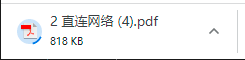
\includegraphics{figs/chunk.PNG}
\end{center}
\caption{分块传输}
\label{chunk}
\end{figure}